\documentclass{article}
\usepackage{amsmath, amssymb}
\usepackage{tcolorbox}
\usepackage{tikz}
\usepackage{geometry}
\usepackage{xcolor}
\usepackage{titlesec}
\usepackage{enumitem}
\usepackage{colortbl}
\usepackage{fancyhdr}
\usepackage{sectsty}
\usepackage{lmodern} % Modern font
\usepackage{microtype} % Improves text appearance
\usepackage{graphicx} % For including images

% Page Geometry
\geometry{a4paper, margin=1in}

% Color Definitions
\definecolor{sectioncolor}{RGB}{60,60,60}
\definecolor{definitioncolor}{RGB}{255,102,0}
\definecolor{tableheadercolor}{RGB}{230,230,230}

% Section Formatting
\sectionfont{\color{sectioncolor}\normalfont\Large\bfseries}
\subsectionfont{\color{sectioncolor}\normalfont\large\bfseries}

% Highlighted Box for Definitions
\newtcolorbox{definitionbox}[1][]{
    colframe=definitioncolor!80,
    colback=definitioncolor!10,
    fonttitle=\bfseries,
    title=#1
}

% Header and Footer
\pagestyle{fancy}
\fancyhf{}
\fancyhead[L]{IB Analysis and Approaches HL2}
\fancyhead[R]{Inverse Trigonometric Functions}
\fancyfoot[C]{\thepage}

% Title
\title{\textbf{IB Analysis and Approaches HL2 \\ Inverse Trigonometric Functions}}
\author{}
\date{}

\begin{document}
\maketitle

% Introduction Section
\section*{Definition \& Purpose}
Functions that reverse the effect of the basic trigonometric functions (sine, cosine, and tangent).

If a trigonometric function takes an angle and gives us a ratio, the inverse trigonometric function takes a ratio and gives back the angle.

% Understanding Trigonometry Section
\section*{Triangle Example}
Suppose we have a right triangle with an angle $\theta$ and sides of length $a$, $b$, and $c$ as shown below.

\begin{center}
    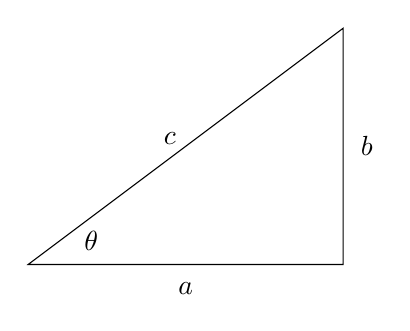
\begin{tikzpicture}
        \draw (0,0) -- (4,0) -- (4,3) -- cycle;
        \node at (2,-0.3) {$a$};
        \node at (4.3,1.5) {$b$};
        \node at (1.8,1.6) {$c$};
        \node at (0.8,0.3) {$\theta$};
    \end{tikzpicture}
\end{center}

In regular trigonometry:
\begin{align*}
    \sin(\theta) & = \frac{b}{c}, \\
    \cos(\theta) & = \frac{a}{c}, \\
    \tan(\theta) & = \frac{b}{a}.
\end{align*}

% Corrected the table formatting for clarity
\begin{center}
    \begin{tabular}{|p{0.35\textwidth}|p{0.25\textwidth}|p{0.25\textwidth}|}
        \hline
        \rowcolor{tableheadercolor}
        \textbf{Trigonometric Function} & \textbf{Domain}        & \textbf{Range}                             \\
        \hline
        $\arcsin(x)$                    & $-1 \leq x \leq 1$     & $-\frac{\pi}{2} \leq y \leq \frac{\pi}{2}$ \\
        \hline
        $\arccos(x)$                    & $-1 \leq x \leq 1$     & $0 \leq y \leq \pi$                        \\
        \hline
        $\arctan(x)$                    & $-\infty < x < \infty$ & $-\frac{\pi}{2} < y < \frac{\pi}{2}$       \\
        \hline
    \end{tabular}
\end{center}

\subsection*{Domain and Range Visualization}

\begin{center}
    \includegraphics[width=\textwidth]{Screenshot 2024-05-14 192525.png}
\end{center}

\section*{Example Problems}

\begin{enumerate}

    \item \textbf{Find, where possible, the exact solutions of}:
          \begin{enumerate}
              \item \(\arctan x = \frac{\pi}{6}\)

                    \textbf{Solution:}
                    \[
                        \tan\left(\frac{\pi}{6}\right) = \frac{1}{\sqrt{3}} \implies x = \frac{1}{\sqrt{3}}
                    \]

              \item \(\arccos(x - 1) = \frac{\pi}{4}\)

                    \textbf{Solution:}
                    \[
                        x - 1 = \cos\left(\frac{\pi}{4}\right) = \frac{\sqrt{2}}{2}
                    \]
                    Solving for \(x\):
                    \[
                        x = \frac{\sqrt{2}}{2} + 1
                    \]

              \item \(\arcsin x = \frac{\pi}{6}\)

                    \textbf{Solution:}
                    \[
                        x = \sin\left(\frac{\pi}{6}\right) = \frac{1}{2}
                    \]
          \end{enumerate}

    \item \textbf{Find the invariant point for the inverse transformation from}:
          \begin{enumerate}
              \item \(y = \sin x \) to \(y = \arcsin x\)

                    \textbf{Solution:}
                    Since both functions need to be equal, we get:
                    \[
                        \sin(x) = x
                    \]
                    The solution needs to be in the range of \(\arcsin(x)\), which is \([-1, 1]\). Therefore, the invariant point is:
                    \[
                        (0, 0)
                    \]

              \item \(y = \tan x \) to \(y = \arctan x\)

                    \textbf{Solution:}
                    Since both functions must be equal, we get:
                    \[
                        \tan(x) = x
                    \]
                    The solution needs to be in the range of \(\arctan(x)\), which is \((-\infty, \infty)\). Therefore, the invariant point is:
                    \[
                        (0, 0)
                    \]
          \end{enumerate}
\end{enumerate}

\section*{Key Takeaways}
\begin{definitionbox}[Inverse Trigonometric Functions]
    \begin{itemize}
        \item $\arcsin(x)$: Inverse of $\sin(x)$. Domain: $-1 \leq x \leq 1$, Range: $-\frac{\pi}{2} \leq y \leq \frac{\pi}{2}$.
        \item $\arccos(x)$: Inverse of $\cos(x)$. Domain: $-1 \leq x \leq 1$, Range: $0 \leq y \leq \pi$.
        \item $\arctan(x)$: Inverse of $\tan(x)$. Domain: $-\infty < x < \infty$, Range: $-\frac{\pi}{2} < y < \frac{\pi}{2}$.
    \end{itemize}
\end{definitionbox}

\end{document}
